
%
The {\em parallel vectors} (PV) operator \cite{Peikert1999} is a generic and
widely spread concept in visualization.
%
Given two 3D vector fields $ \vv_1, \vv_2$, the PV operator delivers all points
in the 3D domain where $ \vv_1$ and $\vv_2$ are linearly dependent.
%
It is known that the PV operator delivers structurally stable lines which we
call PV lines.
%
Inserting different concrete vector fields into it, the PV operator has been
proven to be a generic tool to extract vortex core lines or bifurcation lines.
%
Several numerical methods to extract PV lines have been developed.
%

%
In this paper we introduce the new concept of the {\em parallel eigenvectors}
(PEV) operator of two (not necessarily symmetric) 3D second order tensor fields.
%
Let $\mS(\vx)$ and $\mT(\vx)$ be two such tensor fields.
%
Then the PEV operator collects all points where $\mS$ and $\mT$ have parallel
real eigenvectors:
%
\begin{equation}
    \mbox{PEV}(\mS,\mT) = \{ \vx \;|\; \exists \;\ve,
        \ve \;\mbox{real and eigenvector of both} \;\mS(\vx),\mT(\vx) \}.
\end{equation}
%
In order to establish this operator, we make the following contributions:
%
\begin{itemize}
    \item
    We study properties of the PEV operator.
    %
    In particular, we show that the PEV operator produces structurally stable 3D
    line structures.
    %
    We also study the behavior of these lines in regions where one of the tensor
    fields is in transition between real and imaginary eigenvectors.
    %
    \item
    We present a numerical algorithm to extract PEV lines in piecewise linear
    tensor fields.
    %
    The main idea is to do a search not only in 3D space but simultaneously in
    3D space and the space of all possible eigenvectors.
    %
    \item
    We apply the PEV operator in two scenarios:
    %
    the comparative visualization of two aligned DT-MRI data sets,
    %
    and the extraction of vortex core lines based on the Jacobian of a velocity
    field and the Jacobian of its acceleration field.
\end{itemize}
%

\subsection*{Relation to the PV operator}
%
At first glance, the PEV operator seems to be a straightforward extension of the
classical PV operator:
%
given two tensor fields $\mS, \mT$, we consider the eigenvector fields just as
vector fields and apply the PV operator to them.
%
Such naive approach cannot give stable results for the PEV operator because of
the following reasons:
%
\begin{itemize}
    \item
    Undefined length and orientation of eigenvectors:\\
    %
    Tensor data is usually given on a grid and requires interpolation within the
    cells.
    %
    While interpolation of the tensor components is straightforward,
    interpolation of the eigenvectors is tricky because of the undefined
    orientation and length.
    %
    In fact, heuristic assumptions about orientation and length are necessary
    that influence the interpolation.
    %
    \item
    Discontinuities in eigenvectors:\\
    %
    A small change of a tensor does not necessarily result in a small change of
    the eigenvectors.
    %
    In fact, in nearly isotropic regions (i.e., where two real eigenvalues are
    similar), a small change of the tensor may result in a dramatic change of
    the eigenvector.
    %
    Moreover, in regions of transition between real and imaginary eigenvalues
    (i.e., in neighborhoods containing both tensors with all real eigenvalues
    and tensors with imaginary eigenvalues), a small change of the tensor can
    result in a sudden appearance/disappearance of real eigenvectors.
    %
    \item
    Existence of multiple eigenvectors:\\
    %
    Regions with three real eigenvectors require a decision on which of them to
    use for the PV operator.
    %
    In particular for interpolation it has be be made sure that the "right"
    eigenvectors are interpolated -- a decision that is particularly non-unique
    in nearly isotropic regions.
    %
\end{itemize}
%
Some of the problems mentioned above could be tackled by local heuristics (for
instance, the orientation of the eigenvectors at the vertices of a cell could
be chosen as consistent as possible).
%
However, especially the second point shows that eigenvectors show a
fundamentally different behavior than normal vector fields for which the PV
operator is designed.
%
Because of this, new algorithms or the extraction of PEV lines are necessary.
%

%
There are a number of approaches in vortex extraction where a vector field $\vv$
is compared with the eigenvectors of a tensor field $\mS$.
%
This "mixed case" (eigenvector parallel to a vector) can be easily reduced to
the classical PV operator by comparing $\vv$ and $\mS\,\vv$.
%
The challenging case considered in this paper is the comparison of the
eigenvectors of two tensor fields.

%
In the following, we first give an overview of related work and introduce the
notation used throughout the paper.
%
We then give some theoretical properties of the PEV operator in
\autoref{sec:tcl_theory}, before detailing our algorithm for finding PEV lines in
piecewise linear tensor fields in \autoref{sec:extracting_pev_lines}.
%
In \autoref{sec:tcl_results}, we present our results for mechanical stress tensor
data as well as on the derivative of the flow map of different flows.
%
We close with a discussion and future work in \autoref{sec:tcl_discussion} and
\autoref{sec:tcl_limitations}.
%

%
\begin{figure*}[tb]
    \centering
    \begin{tabular}{cccc}
        \rule[-0.5cm]{0pt}{0pt}
        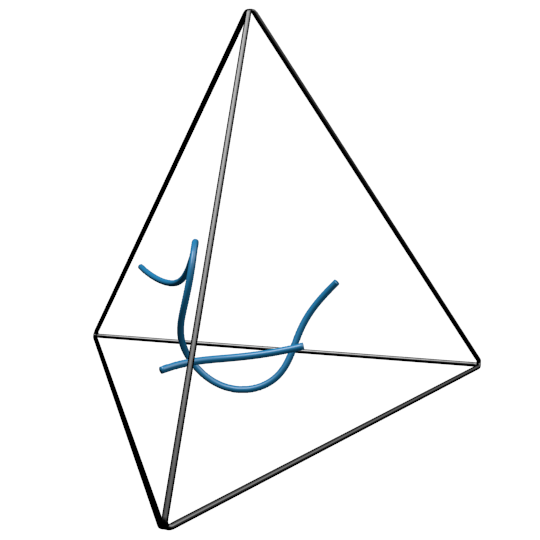
\includegraphics[width=0.45\columnwidth]{figures/Rand_general_1.png} &
        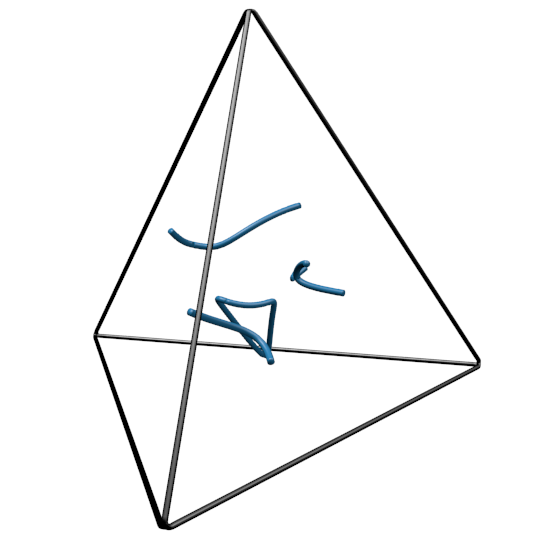
\includegraphics[width=0.45\columnwidth]{figures/Rand_general_2.png} &
        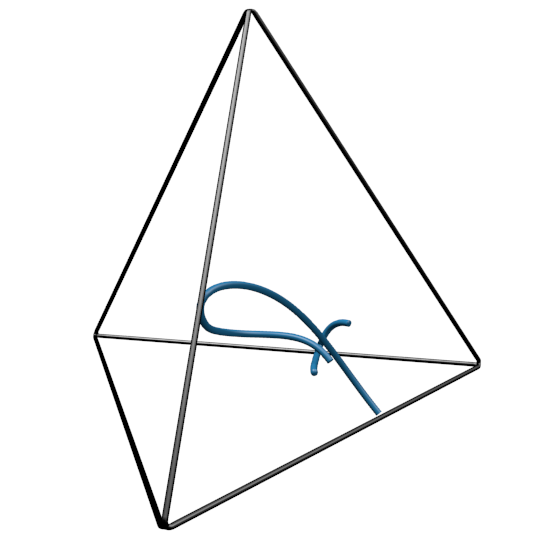
\includegraphics[width=0.45\columnwidth]{figures/Rand_general_3.png} &
        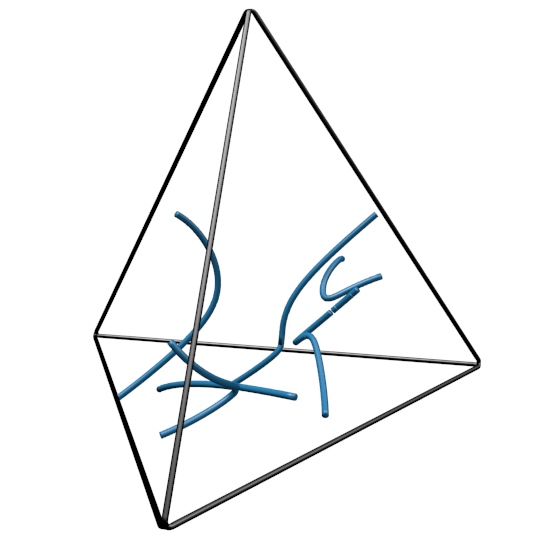
\includegraphics[width=0.45\columnwidth]{figures/Rand_general_4.png} \\
        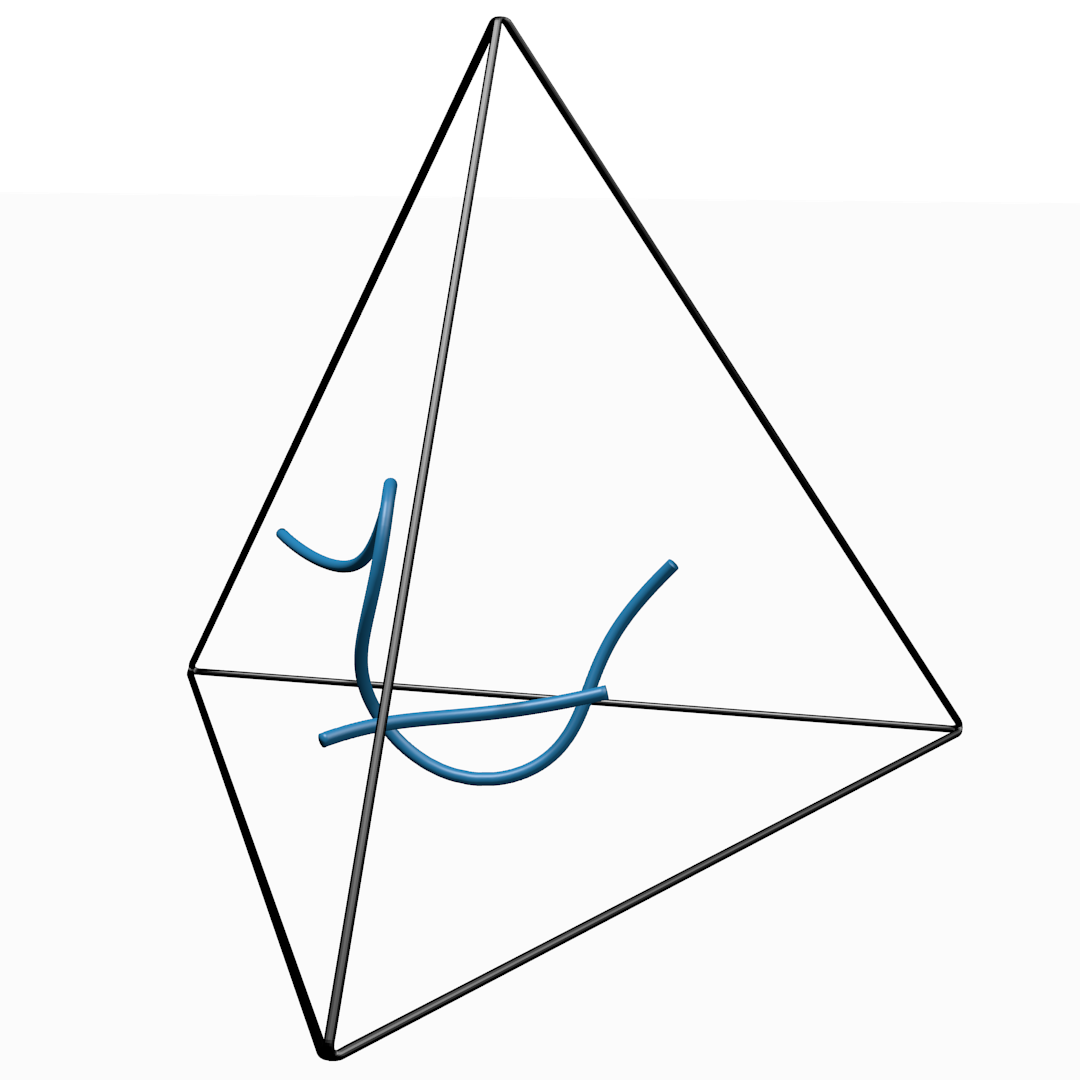
\includegraphics[width=0.45\columnwidth]{figures/Rand_symm_1.png} &
        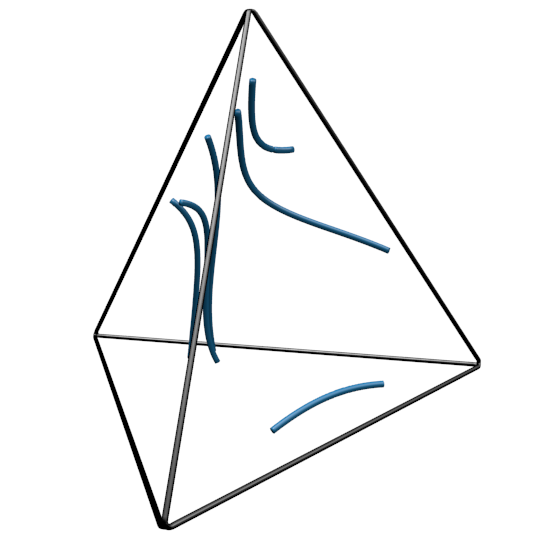
\includegraphics[width=0.45\columnwidth]{figures/Rand_symm_2.png} &
        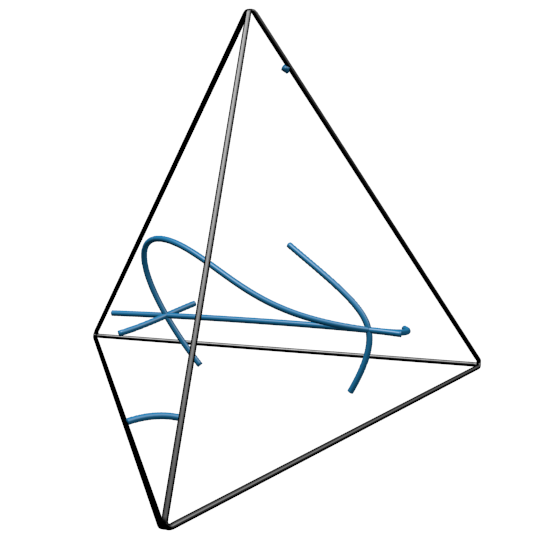
\includegraphics[width=0.45\columnwidth]{figures/Rand_symm_3.png} &
        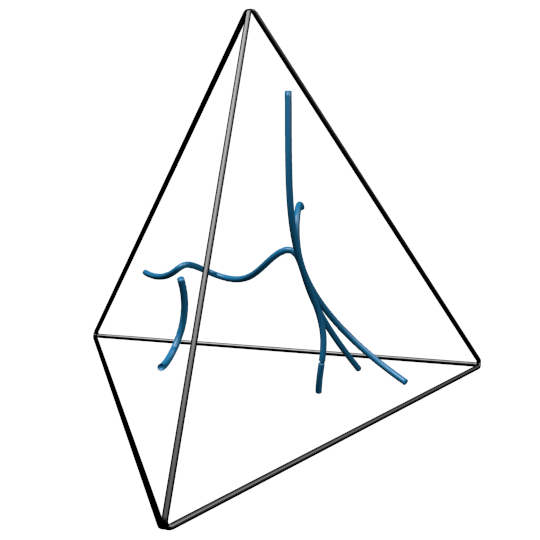
\includegraphics[width=0.45\columnwidth]{figures/Rand_symm_4.png}
    \end{tabular}
    \caption{PEV lines in pairs of random linear tensor fields. Top: General
             tensors. Bottom: Symmetric tensors. Symmetric tensors generally
             produce more lines, as they always have three real eigenvectors.
             General tensor PEV lines generally do not intersect, while it is
             common for symmetric tensor PEV lines to do so. If they do,
             three PEV lines always intersect at once, as their eigenvectors
             are orthogonal.}
    \label{fig:rand_lines}
\end{figure*}
%
% section introduction (end)